\documentclass[a4paper,UTF8]{article}
\usepackage{ctex}
\usepackage[margin=1.25in]{geometry}
\usepackage{color}
\usepackage{graphicx}
\usepackage{amssymb}
\usepackage{amsmath}
\usepackage{amsthm}
\usepackage{enumerate}
\usepackage{bm}
\usepackage{hyperref}
\usepackage{epsfig}
\usepackage{color}
\usepackage{mdframed}  
\usepackage{lipsum}
\usepackage{graphicx}
\newmdtheoremenv{thm-box}{Theorem}
\newmdtheoremenv{prop-box}{Proposition}
\newmdtheoremenv{def-box}{定义}

\usepackage{listings}
\usepackage{xcolor}
\lstset{
	numbers=left, 
	numberstyle= \tiny, 
	keywordstyle= \color{ blue!70},
	commentstyle= \color{red!50!green!50!blue!50}, 
	frame=shadowbox, % 阴影效果
	rulesepcolor= \color{ red!20!green!20!blue!20} ,
	escapeinside=``, % 英文分号中可写入中文
	xleftmargin=2em,xrightmargin=2em, aboveskip=1em,
	framexleftmargin=2em
} 

\usepackage{booktabs}

\setlength{\evensidemargin}{.25in}
\setlength{\textwidth}{6in}
\setlength{\topmargin}{-0.5in}
\setlength{\topmargin}{-0.5in}
% \setlength{\textheight}{9.5in}
%%%%%%%%%%%%%%%%%%此处用于设置页眉页脚%%%%%%%%%%%%%%%%%%
\usepackage{fancyhdr}                                
\usepackage{lastpage}                                           
\usepackage{layout}                                             
\footskip = 10pt 
\pagestyle{fancy}                    % 设置页眉                 
\lhead{2018年春季}                    
\chead{机器学习导论}                                                
% \rhead{第\thepage/\pageref{LastPage}页} 
\rhead{作业二}                                                                                               
\cfoot{\thepage}                                                
\renewcommand{\headrulewidth}{1pt}  			%页眉线宽,设为0可以去页眉线
\setlength{\skip\footins}{0.5cm}    			%脚注与正文的距离           
\renewcommand{\footrulewidth}{0pt}  			%页脚线宽,设为0可以去页脚线

\makeatletter 									%设置双线页眉                                        
\def\headrule{{\if@fancyplain\let\headrulewidth\plainheadrulewidth\fi%
\hrule\@height 1.0pt \@width\headwidth\vskip1pt	%上面线为1pt粗  
\hrule\@height 0.5pt\@width\headwidth  			%下面0.5pt粗            
\vskip-2\headrulewidth\vskip-1pt}      			%两条线的距离1pt        
 \vspace{6mm}}     								%双线与下面正文之间的垂直间距              
\makeatother  

%%%%%%%%%%%%%%%%%%%%%%%%%%%%%%%%%%%%%%%%%%%%%%
\numberwithin{equation}{section}
%\usepackage[thmmarks, amsmath, thref]{ntheorem}
\newtheorem{theorem}{Theorem}
\newtheorem*{definition}{Definition}
\newtheorem*{solution}{Solution}
\newtheorem*{prove}{Proof}
\newcommand{\indep}{\rotatebox[origin=c]{90}{$\models$}}

\usepackage{multirow}

%--

%--
\begin{document}
\title{机器学习导论\\
作业二}
\author{151220097, 孙旭东, 248381185@qq.com}
\maketitle

\section{[25pts] Multi-Class Logistic Regression}
教材的章节3.3介绍了对数几率回归解决二分类问题的具体做法。假定现在的任务不再是二分类问题,而是多分类问题,其中标记$y\in\{1,2\dots,K\}$。请将对数几率回归算法拓展到该多分类问题。

\begin{enumerate}[(1)]
	\item \textbf{[15pts]} 给出该对率回归模型的“对数似然”(log-likelihood);
	\item \textbf{[10pts]} 计算出该“对数似然”的梯度。
\end{enumerate}

提示1:假设该多分类问题满足如下$K-1$个对数几率,
\begin{eqnarray*}
	\ln\frac{p(y=1|\mathbf{x})}{p(y=K|\mathbf{x})}&=&\mathbf{w}_1^\mathrm{T}\mathbf{x}+b_1\\
	\ln\frac{p(y=2|\mathbf{x})}{p(y=K|\mathbf{x})}&=&\mathbf{w}_2^\mathrm{T}\mathbf{x}+b_2\\
	&\dots&\\
	\ln\frac{p(y={K-1}|\mathbf{x})}{p(y=K|\mathbf{x})}&=&\mathbf{w}_{K-1}^\mathrm{T}\mathbf{x}+b_{K-1}
\end{eqnarray*}

提示2:定义指示函数$\mathbb{I}(\cdot)$,
$$\mathbb{I}(y=j)=
\begin{cases}
1& \text{若$y$等于$j$}\\
0& \text{若$y$不等于$j$}
\end{cases}$$

\begin{solution}
\begin{enumerate}
	
\item
因为
\begin{equation}
	\ln\frac{p(y=i|\mathbf{x})}{p(y=K|\mathbf{x})}=\mathbf{w}_i^\mathrm{T}\mathbf{x}+b_i
\end{equation} 	
所以
\begin{equation}
	\frac{p(y=i|\mathbf{x})}{p(y=K|\mathbf{x})} = e^{\mathbf{w}_i^\mathrm{T}\mathbf{x}+b_i}
\end{equation}
进一步有
\begin{equation}
	\frac{1-p(y=K|\mathbf{x})}{p(y=K|\mathbf{x})} = \sum_{i=1}^{K-1}e^{\mathbf{w}_i^\mathrm{T}\mathbf{x}+b_i}
\end{equation}
所以可得
\begin{equation}
	p(y=K|\mathbf{x}) = \frac{1}{1 + \sum_{i=1}^{K-1}e^{\mathbf{w}_i^\mathrm{T}\mathbf{x}+b_i}}
\end{equation}
由此可得当$k\neq K$
\begin{equation}
	p(y=k|\mathbf{x}) = \frac{e^{\mathbf{w}_k^\mathrm{T}\mathbf{x}+b_k}}{1 + \sum_{i=1}^{K-1}e^{\mathbf{w}_i^\mathrm{T}\mathbf{x}+b_i}}
\end{equation}
综上所述,我们有
\begin{equation}
		p(y=k|\mathbf{x}) = \begin{cases}
		\frac{e^{\mathbf{w}_k^\mathrm{T}\mathbf{x}+b_k}}{1 + \sum_{i=1}^{K-1}e^{\mathbf{w}_i^\mathrm{T}\mathbf{x}+b_i}} & k\neq K;\\
		\frac{1}{1 + \sum_{i=1}^{K-1}e^{\mathbf{w}_i^\mathrm{T}\mathbf{x}+b_i}} & k = K.
		\end{cases}
\end{equation}
进一步可以得到
\begin{equation}
p(y_i|\mathbf{x}_i;\mathbf{w}_1, \mathbf{w}_2,...,\mathbf{w}_{K-1}, b_1, b_2,...,b_{K-1}) = \sum_{j=1}^{K}\mathbb{I}(y_i=j) p(y_i=j|\mathbf{x}_i;\mathbf{w}_1, ...,\mathbf{w}_{K-1}, b_1, ...,b_{K-1})
\end{equation}
通过观察可以发现,在$\mathbb{I}(y_i=j)\ (1 \leq j \leq K)$这$K$个式子中,有且仅有一个可以取1,其他全部为0。根据这个性质,再对概率取对数,可以得到
\begin{equation}
\begin{aligned}
&\ln p(y_i|\mathbf{x}_i;\mathbf{w}_1, \mathbf{w}_2,...,\mathbf{w}_{K-1}, b_1, b_2,...,b_{K-1})\\ 
=& \ln \sum_{j=1}^{K}\mathbb{I}(y_i=j) p(y_i=j|\mathbf{x}_i;\mathbf{w}_1,...,\mathbf{w}_{K-1}, b_1,...,b_{K-1})\\
=& \sum_{j=1}^{K}\mathbb{I}(y_i=j)\ln p(y_i=j|\mathbf{x}_i;\mathbf{w}_1,...,\mathbf{w}_{K-1}, b_1,...,b_{K-1})
\end{aligned}
\end{equation}
我们假设总共有$m$个样例,下面计算对数似然
\begin{equation}
\begin{aligned}
&\ell(\mathbf{w}_1, \mathbf{w}_2,...,\mathbf{w}_{K-1}, b_1, b_2,...,b_{K-1})\\
=& \sum_{i=1}^{m}\ln p(y_i|\mathbf{x}_i;\mathbf{w}_1,...,\mathbf{w}_{K-1}, b_1,...,b_{K-1})\\
=& \sum_{i=1}^{m}\sum_{j=1}^{K}\mathbb{I}(y_i=j)\ln p(y_i=j|\mathbf{x}_i;\mathbf{w}_1,...,\mathbf{w}_{K-1}, b_1,...,b_{K-1})
\end{aligned}
\end{equation}
为了便于讨论,令$\boldsymbol{\beta}_j = (\mathbf{w}_j; b_j)$以及$\hat{\mathbf{x}}_i = (\mathbf{x}_i; 1)$,现在$\mathbf{w}_j^\mathrm{T}\mathbf{x}_i+b_j$可以简写为$\boldsymbol{\beta}_j^\mathrm{T}\hat{\mathbf{x}}_i$,并且因为只是改变了符号,所以对数极大似然可以写成如下形式
\begin{equation}
\begin{aligned}
&\ell(\boldsymbol{\beta}_1, \boldsymbol{\beta}_2,...,\boldsymbol{\beta}_{K-1})\\
=& \ell(\mathbf{w}_1, \mathbf{w}_2,...,\mathbf{w}_{K-1}, b_1, b_2,...,b_{K-1}) \\
=& \sum_{i=1}^{m}\sum_{j=1}^{K}\mathbb{I}(y_i=j)\ln p(y_i=j|\mathbf{x}_i;\mathbf{w}_1,...,\mathbf{w}_{K-1}, b_1,...,b_{K-1})\\
=&\sum_{i=1}^{m}\sum_{j=1}^{K}\mathbb{I}(y_i=j)\ln p(y_i=j|\hat{\mathbf{x}}_i;\boldsymbol{\beta}_1, \boldsymbol{\beta}_2,...,\boldsymbol{\beta}_{K-1})
\end{aligned}
\end{equation}
根据以上讨论,最终对数似然求解如下
\begin{equation}
\begin{aligned}
&\ell(\boldsymbol{\beta}_1, \boldsymbol{\beta}_2,...,\boldsymbol{\beta}_{K-1}) = \sum_{i=1}^{m}\sum_{j=1}^{K}\mathbb{I}(y_i=j)\ln p(y_i=j|\hat{\mathbf{x}}_i;\boldsymbol{\beta}_1, \boldsymbol{\beta}_2,...,\boldsymbol{\beta}_{K-1})\\
=& \sum_{i=1}^{m}\sum_{j=1}^{K-1}\mathbb{I}(y_i=j)\ln \frac{e^{\boldsymbol{\beta}_j^\mathrm{T}\hat{\mathbf{x}}_i}}{1 + \sum_{t=1}^{K-1}e^{\boldsymbol{\beta}_t^\mathrm{T}\hat{\mathbf{x}}_i}} + \sum_{i=1}^{m}\mathbb{I}(y_i=K)\ln\frac{1}{1 + \sum_{t=1}^{K-1}e^{\boldsymbol{\beta}_t^\mathrm{T}\hat{\mathbf{x}}_i}}\\
=& \sum_{i=1}^{m}\sum_{j=1}^{K-1}\mathbb{I}(y_i=j)(\boldsymbol{\beta}_j^\mathrm{T}\hat{\mathbf{x}}_i- \ln (1 + \sum_{t=1}^{K-1}e^{\boldsymbol{\beta}_t^\mathrm{T}\hat{\mathbf{x}}_i})) - \sum_{i=1}^{m}\mathbb{I}(y_i=K)\ln(1 + \sum_{t=1}^{K-1}e^{\boldsymbol{\beta}_t^\mathrm{T}\hat{\mathbf{x}}_i})\\
=&\sum_{i=1}^{m}\sum_{j=1}^{K-1}\mathbb{I}(y_i=j)(\boldsymbol{\beta}_j^\mathrm{T}\hat{\mathbf{x}}_i) - \sum_{i=1}^{m}\ln(1 + \sum_{t=1}^{K-1}e^{\boldsymbol{\beta}_t^\mathrm{T}\hat{\mathbf{x}}_i})
\end{aligned}
\end{equation}
综上所述
\begin{equation}
\ell(\boldsymbol{\beta}_1, \boldsymbol{\beta}_2,...,\boldsymbol{\beta}_{K-1}) = \sum_{i=1}^{m}\sum_{j=1}^{K-1}\mathbb{I}(y_i=j)(\boldsymbol{\beta}_j^\mathrm{T}\hat{\mathbf{x}}_i) - \sum_{i=1}^{m}\ln(1 + \sum_{t=1}^{K-1}e^{\boldsymbol{\beta}_t^\mathrm{T}\hat{\mathbf{x}}_i})
\end{equation}

\item
$\ell(\boldsymbol{\beta}_1, \boldsymbol{\beta}_2,...,\boldsymbol{\beta}_{K-1})$对$\boldsymbol{\beta}_j$求偏导,即可得到对数似然的梯度:
\begin{equation}
\begin{aligned}
\frac{\partial\ell(\boldsymbol{\beta}_1, \boldsymbol{\beta}_2,...,\boldsymbol{\beta}_{K-1})}{\partial\boldsymbol{\beta}_j} 
=& \sum_{i=1}^{m}\mathbb{I}(y_i=j)\hat{\mathbf{x}}_i - \sum_{i=1}^{m}\frac{e^{\boldsymbol{\beta}_j^\mathrm{T}\hat{\mathbf{x}}_i}}{1 + \sum_{t=1}^{K-1}e^{\boldsymbol{\beta}_t^\mathrm{T}\hat{\mathbf{x}}_i}}\hat{\mathbf{x}}_i\\
=& \sum_{i=1}^{m}(\mathbb{I}(y_i=j) - \frac{e^{\boldsymbol{\beta}_j^\mathrm{T}\hat{\mathbf{x}}_i}}{1 + \sum_{t=1}^{K-1}e^{\boldsymbol{\beta}_t^\mathrm{T}\hat{\mathbf{x}}_i}})\hat{\mathbf{x}}_i\\
=& \sum_{i=1}^{m}(\mathbb{I}(y_i=j) - 	p(y_i=j|\hat{\mathbf{x}}_i))\hat{\mathbf{x}}_i
\end{aligned}
\end{equation} 
所以梯度为:
\begin{equation}
\begin{aligned}
&\nabla \ell(\boldsymbol{\beta}_1, \boldsymbol{\beta}_2,...,\boldsymbol{\beta}_{K-1})\\
=&\left(\frac{\partial\ell(\boldsymbol{\beta}_1, \boldsymbol{\beta}_2,...,\boldsymbol{\beta}_{K-1})}{\partial\boldsymbol{\beta}_1},\ ...,\frac{\partial\ell(\boldsymbol{\beta}_1, \boldsymbol{\beta}_2,\ ...,\  \boldsymbol{\beta}_{K-1})}{\partial\boldsymbol{\beta}_{K-1}}\right)\\
=& \left(\sum_{i=1}^{m}(\mathbb{I}(y_i=1) - 	p(y_i=1|\hat{\mathbf{x}}_i))\hat{\mathbf{x}}_i,\ ...,\ \sum_{i=1}^{m}(\mathbb{I}(y_i=K-1) - 	p(y_i=K-1|\hat{\mathbf{x}}_i))\hat{\mathbf{x}}_i\right)
\end{aligned}
\end{equation}
\end{enumerate}	
	
\end{solution}
\newpage


\section{[20pts] Linear Discriminant Analysis}
假设有两类数据,正例独立同分布地从高斯分布$\mathcal{N}(\mu_1,\Sigma_1)$采样得到,负例独立同分布地从另一高斯分布$\mathcal{N}(\mu_2,\Sigma_2)$采样得到,其中参数$\mu_1,\Sigma_1$及$\mu_2,\Sigma_2$均已知。现在,我们定义“最优分类”:若对空间中的任意样本点,分别计算已知该样本采样于正例时该样本出现的概率与已知该样本采样于负例时该样本出现的概率后,取概率较大的所采类别作为最终预测的类别输出,则我们说这样的分类方式满足“最优分类”性质。

试证明:当两类数据的分布参数$\Sigma_1=\Sigma_2=\Sigma$时,线性判别分析 (LDA)方法满足“最优分类”性质。(提示:找到满足最优分类性质的分类平面。)
\begin{solution}
~\\
由于正例和负例服从高斯分布,我们用$y_1$表示正例,用$y_2$表示负例,所以可知:\\
已知该样本采样于正例,该样本出现的概率为:\\
\begin{equation}
p(\mathbf{x} = x \mid \mathbf{y} = y_1) = \frac{1}{(2\pi)^{\frac{n}{2}}\lvert \Sigma \rvert^{\frac{1}{2}}}\exp(-\frac{1}{2}(x - \mu_1)^\mathrm{T}\Sigma^{-1}(x - \mu_1)
)
\end{equation}
已知该样本采样于负例,该样本出现的概率为:\\
\begin{equation}
p(\mathbf{x} = x \mid \mathbf{y} = y_2) = \frac{1}{(2\pi)^{\frac{n}{2}}\lvert \Sigma \rvert^{\frac{1}{2}}}\exp(-\frac{1}{2}(x - \mu_2)^\mathrm{T}\Sigma^{-1}(x - \mu_2)
)
\end{equation}
对概率取对数,可得(注意到$\Sigma$是对称矩阵)
\begin{equation}
\begin{aligned}
\ln p(\mathbf{x} = x \mid \mathbf{y} = y_i) 
=&- \ln((2\pi)^{\frac{n}{2}}\lvert \Sigma \rvert^{\frac{1}{2}}) - \frac{1}{2}(x - \mu_i)^\mathrm{T}\Sigma^{-1}(x - \mu_i)\\
=&- \ln((2\pi)^{\frac{n}{2}}\lvert \Sigma \rvert^{\frac{1}{2}}) - \frac{1}{2}(x^\mathrm{T}\Sigma^{-1}x + \mu_i^\mathrm{T}\Sigma^{-1}\mu_i - 2x^{\mathrm{T}}\Sigma^{-1}\mu_i)\\
=&- \ln((2\pi)^{\frac{n}{2}}\lvert \Sigma \rvert^{\frac{1}{2}}) - \frac{1}{2}x^\mathrm{T}\Sigma^{-1}x - \frac{1}{2} \mu_i^\mathrm{T}\Sigma^{-1}\mu_i + x^{\mathrm{T}}\Sigma^{-1}\mu_i
\end{aligned}
\end{equation}
注意到$\frac{1}{2}x^\mathrm{T}\Sigma^{-1}x$和$ \ln((2\pi)^{\frac{n}{2}}\lvert \Sigma \rvert^{\frac{1}{2}})$都是和$i$无关的,所以为了方便之后的计算,令$C = - \ln((2\pi)^{\frac{n}{2}}\lvert \Sigma \rvert^{\frac{1}{2}}) - \frac{1}{2}x^\mathrm{T}\Sigma^{-1}x$,可得
\begin{equation}
\ln p(\mathbf{x} = x \mid \mathbf{y} = y_i)  = C - \frac{1}{2} \mu_i^\mathrm{T}\Sigma^{-1}\mu_i + x^{\mathrm{T}}\Sigma^{-1}\mu_i 
\end{equation}
所以有:
\begin{equation}
\ln p( \mathbf{x} = x \mid \mathbf{y} = y_1) = C - \frac{1}{2} \mu_1^\mathrm{T}\Sigma^{-1}\mu_1 + x^{\mathrm{T}}\Sigma^{-1}\mu_1 
\end{equation}
\begin{equation}
\ln p(\mathbf{x} = x \mid \mathbf{y} = y_2) = C - \frac{1}{2} \mu_2^\mathrm{T}\Sigma^{-1}\mu_2 + x^{\mathrm{T}}\Sigma^{-1}\mu_2 
\end{equation}
如果令$(2.5)$和$(2.6)$相减,可得平面方程:
\begin{equation}
	f(x) = x^{\mathrm{T}}\Sigma^{-1}(\mu_1 - \mu_2) - \frac{1}{2}(\mu_1^\mathrm{T}\Sigma^{-1}\mu_1 - \mu_2^\mathrm{T}\Sigma^{-1}\mu_2)
\end{equation}
通过观察易得:\\
当$f(x) = 0$时,$p( \mathbf{x} = x \mid \mathbf{y} = y_1) = p( \mathbf{x} = x \mid \mathbf{y} = y_2)$;\\
当$f(x) > 0$时,$p( \mathbf{x} = x \mid \mathbf{y} = y_1) > p( \mathbf{x} = x \mid \mathbf{y} = y_2)$;\\
当$f(x) < 0$时,$p( \mathbf{x} = x \mid \mathbf{y} = y_1) < p( \mathbf{x} = x \mid \mathbf{y} = y_2)$;\\\\
现在再考虑LDA。根据LDA的定义,所有样例将要被映射到$w$上,$w = S^{-1}_w(\mu_1 - \mu_2)$,同时$S^{-1}_w = \Sigma_1 + \Sigma_2 = 2\Sigma$,所以$w = 2\Sigma^{-1}(\mu_1 - \mu_2)$,这与分类平面的法向量同向。考虑到LDA将所有样本映射到$w$上,所以需要一个阈值来作为正例和负例的分界。设置阈值为$\mu_1^\mathrm{T}\Sigma^{-1}\mu_1 - \mu_2^\mathrm{T}\Sigma^{-1}\mu_2$。\\\\
LDA分类器的预测过程为:\\
对于向量$x$,将其映射到$w = 2\Sigma^{-1}(\mu_1 - \mu_2)$上,得到标量$2x^{\mathrm{T}}\Sigma^{-1}(\mu_1 - \mu_2)$,如果$2x^{\mathrm{T}}\Sigma^{-1}(\mu_1 - \mu_2) > \mu_1^\mathrm{T}\Sigma^{-1}\mu_1 - \mu_2^\mathrm{T}\Sigma^{-1}\mu_2$,则预测为正例,反之预测为负例。现在来证明这个LDA分类器满足最优分类性质。\\\\
根据平面方程$f(x)$的性质以及LDA分类器的定义,可以得到:\\
在比较$2x^{\mathrm{T}}\Sigma^{-1}(\mu_1 - \mu_2)$和$\mu_1^\mathrm{T}\Sigma^{-1}\mu_1 - \mu_2^\mathrm{T}\Sigma^{-1}\mu_2$时,有以下两种情况(此处忽略相等的情况,但不影响证明正确性):\\\\
情况一:$2x^{\mathrm{T}}\Sigma^{-1}(\mu_1 - \mu_2) > \mu_1^\mathrm{T}\Sigma^{-1}\mu_1 - \mu_2^\mathrm{T}\Sigma^{-1}\mu_2$,此时有
\begin{equation}
	x^{\mathrm{T}}\Sigma^{-1}(\mu_1 - \mu_2) - \frac{1}{2}(\mu_1^\mathrm{T}\Sigma^{-1}\mu_1 - \mu_2^\mathrm{T}\Sigma^{-1}\mu_2) > 0
\end{equation}
也就是说$f(x) > 0$,根据平面方程定义,此时
\begin{equation}
p(\mathbf{x} = x \mid \mathbf{y} = y_1) > p(\mathbf{x} = x \mid \mathbf{y} = y_2)
\end{equation}
也就是说“已知$x$采样于正例,$x$出现的概率”大于“已知$x$采样于负例,$x$出现的概率”。而根据LDA分类器的定义,此时会把$x$预测为正例。\\\\
情况二:$2x^{\mathrm{T}}\Sigma^{-1}(\mu_1 - \mu_2) < \mu_1^\mathrm{T}\Sigma^{-1}\mu_1 - \mu_2^\mathrm{T}\Sigma^{-1}\mu_2$,此时有
\begin{equation}
x^{\mathrm{T}}\Sigma^{-1}(\mu_1 - \mu_2) - \frac{1}{2}(\mu_1^\mathrm{T}\Sigma^{-1}\mu_1 - \mu_2^\mathrm{T}\Sigma^{-1}\mu_2) < 0
\end{equation}
也就是说$f(x) < 0$,根据平面方程定义,此时
\begin{equation}
p(\mathbf{x} = x \mid \mathbf{y} = y_1) < p(\mathbf{x} = x \mid \mathbf{y} = y_2)
\end{equation}
也就是说“已知$x$采样于正例,$x$出现的概率”小于“已知$x$采样于负例,$x$出现的概率”。而根据LDA分类器的定义,此时会把$x$预测为负例。\\\\
综合两种情况可得,LDA分类器满足“若对空间中的任意样本点,分别计算已知该样本采样于正例时该样本出现的概率与已知该样本采样于负例时该样本出现的概率后,取概率较大的所采类别作为最终预测的类别输出”。\\
综上所述,LDA方法满足最优分类性质。\\\\
参考资料:\\
1. Izenman A.J. (2013) Modern Multivariate Statistical Techniques\\
2. Christopher M. Bishop (2016) Pattern Recognition and Machine Learning\\
\end{solution}
\newpage



\section{[55+10*pts] Logistic Regression Programming}
在本题中,我们将初步接触机器学习编程,首先我们需要初步了解机器学习编程的主要步骤,然后结合对数几率回归,在UCI数据集上进行实战。机器学习编程的主要步骤可参见\href{http://blog.csdn.net/cqy_chen/article/details/78690975}{博客}。

本次实验选取UCI数据集Page Blocks(\href{http://lamda.nju.edu.cn/ml2018/PS2/PS2_dataset.zip}{下载链接})。数据集基本信息如表~\ref{data_inf}所示,此数据集特征维度为10维,共有5类样本,并且类别间样本数量不平衡。

\begin{table}[!h]
	\centering
	\caption{Page Blocks数据集中每个类别的样本数量。}\vspace{3mm}
	\label{data_inf}
	\begin{tabular}{l|cccccc}\hline
		标记     & 1    & 2   & 3  & 4  & 5   & total \\ \hline
		训练集   & 4431 & 292 & 25 & 84 & 103 & 4935  \\
		测试集   & 482  & 37  & 3  & 4  & 12  & 538   \\ \hline
	\end{tabular}
\end{table}

对数几率回归(Logistic Regression, LR)是一种常用的分类算法。面对多分类问题,结合处理多分类问题技术,利用常规的LR算法便能解决这类问题。

\begin{enumerate}[(1)]
    \item \textbf{[5pts]} 此次编程作业要求使用Python 3或者MATLAB编写,请将main函数所在文件命名为~LR\_main.py或者LR\_main.m,效果为运行此文件便能完成整个训练过程,并输出测试结果,方便作业批改时直接调用;	
	\item \textbf{[30pts]} 本题要求编程实现如下实验功能:
	\begin{itemize}
		\item \textbf{[10pts]} 根据《机器学习》3.3节,实现LR算法,优化算法可选择梯度下降,亦可选择牛顿法;
		\item \textbf{[10pts]} 根据《机器学习》3.5节,利用“一对其余”(One vs. Rest, OvR)策略对分类LR算法进行改进,处理此多分类任务;
		\item \textbf{[10pts]} 根据《机器学习》3.6节,在训练之前,请使用“过采样”(oversampling)策略进行样本类别平衡;
	\end{itemize}
	
	

	\item \textbf{[20pts]} 实验报告中报告算法的实现过程(能够清晰地体现 (1) 中实验要求,请勿张贴源码),如优化算法选择、相关超参数设置等,并填写表~\ref{exp_performance},在\url{http://www.tablesgenerator.com/}上能够方便地制作LaTex表格;
	
	\item \textbf{[附加题 10pts]} 尝试其他类别不平衡问题处理策略(尝试方法可以来自《机器学习》也可来自其他参考材料),尽可能提高对少数样本的分类准确率,并在实验报告中给出实验设置、比较结果及参考文献;
\end{enumerate}
\noindent \textbf{[**注意**]} 本次实验除了numpy等数值处理工具包外禁止调用任何开源机器学习工具包,一经发现此实验题分数为0,请将实验所需所有源码文件与作业pdf文件放在同一个目录下,请勿将数据集放在提交目录中。
\newpage
\noindent{\textbf{实验报告.}}
\begin{table}[!h]
	\centering
	\caption{算法在测试数据集上泛化性能测试结果,先报告在每个类别上的查全率和查准率,最后报告在整个测试数据集上的准确率。}\vspace{3mm}
	\label{exp_performance}
	\begin{tabular}{@{}c|cccccc@{}}
		\toprule
		标记     & 1    & 2    & 3    & 4    & 5    & \begin{tabular}[c]{@{}c@{}}准确率\end{tabular} \\ \midrule
		查全率    & 0.92 & 0.92 & 1.00 & 1.00 & 0.67 & \multirow{2}{*}{0.91}                                     \\
		查准率 & 0.99 & 0.80 & 0.33 & 0.44 & 0.26 &  \\ \cmidrule(r){1-7}
	\end{tabular}
\end{table}

\noindent\textbf{实验目的}\\
使用对数几率回归解决多分类问题\\

\noindent\textbf{实验过程}\\
本次程序的实现主要按照以下几个流程:读入数据,过采样,归一化,进行训练,预测数据。其中关键步骤在于过采样和进行训练。\\\\
过采样:\\
过采样的算法采用了smote算法,也就是针对每一个少数类进行过采样。具体的流程为:\\
对于少数类中的每一个样例$\mathbf{x}$,寻找$\mathbf{x}$的k近邻$\mathbf{xnn}_1,\mathbf{xnn}_2,...,\mathbf{xnn}_k$(寻找近邻要用的距离的定义可以有不同,我采用的是欧式距离),然后随机挑选其中一个近邻$\mathbf{xnn}_t$,在该样例和近邻之间插值生成新的样例$\mathbf{xs}$。插值的过程是针对每一个特征去生成新的特征,具体为:规定$\mathbf{x}(i)$表示$\mathbf{x}$的第$i$个特征,那么针对每一个特征:
\begin{equation}
\mathbf{xs}(i) = \mathbf{x}(i) + gap*(\mathbf{x}(i) - \mathbf{xnn}_t(i))
\end{equation}
其中$gap$是随机生成的在0和1之间的随机数。这样就成功生成了一个新的样例。如果要把少数类扩大N倍,那么重复上述过程N次,即可完成过采样操作。\\\\
训练过程:\\
因为是多分类问题,所以训练的过程主要采用了One vs Rest的思想,每次把一个类作为正例,其余所有类作为反例,按照二分类问题的方法来训练出一组针对正例类的参数,这样针对每一个类别进行一次训练,共计训练出5个模型。\\
在训练的过程中,需要首先确定模型的cost function,我所采用的cost function是
\begin{equation}
J = \frac{1}{m}\sum_{i=1}^{m}(-y_i\log(h(\mathbf{x}_i)) + (1-y_i)\log(1-h(\mathbf{x}_i)))
\end{equation}
其中
\begin{equation}
h(\mathbf{x}) = \frac{1}{1 + \exp(-\boldsymbol{\theta}^\mathrm{T}\mathbf{x})}
\end{equation}
接下来只要对$J$最小化,求得对应的$\boldsymbol{\theta}$,就完成了对这个类的训练。\\
具体的优化算法我采用的是梯度下降,大致流程为首先计算出$J$对于$\theta$的偏导数:
\begin{equation}
\frac{\partial J}{\partial \boldsymbol{\theta}} = \frac{1}{m}\sum_{i=1}^{m}(h(\mathbf{x}_i )- y_i)\mathbf{x}_i
\end{equation}
梯度下降的迭代公式为
\begin{equation}
\boldsymbol{\theta}^k = \boldsymbol{\theta}^{k-1} - \alpha\frac{\partial J}{\partial \boldsymbol{\theta}^{k-1}}
\end{equation}
其中$\alpha$是下降步长。\\
训练结束得到最终的$\boldsymbol{\theta}$之后,就可以用$\boldsymbol{\theta}$来对测试集做预测了。\\\\
预测过程:\\
考虑到这是一个多分类问题,所以在进行预测的时候实际上需要得到多个预测值然后进行比较。本题是5类,所以根据上面的训练过程会得到5个对应的$\boldsymbol{\theta}$,记为$\mathbf{T} = (\boldsymbol{\theta}^{(1)}, \boldsymbol{\theta}^{(2)}, ..., \boldsymbol{\theta}^{(5)})$,对于每一个测试样例$(\mathbf{x}; y)$,计算$h_i(\mathbf{x}) = \frac{1}{1 + \exp(-{\boldsymbol{\theta}^{(i)}}^\mathrm{T}\mathbf{x})}$,得到$k=arg \max_i h_i(\mathbf{x})$,那么就预测样例$(\mathbf{x}; y)$属于$k$类。\\\\
归一化:\\
考虑到不同特征之间差异较大,有的特征大小可以达到几千,有的不到1,所以进行了归一化的处理,具体操作为针对每一种特征,计算其均值$\mu$和方差$\sigma$,然后对每一个特征值$t$,构造$t' = (t-\mu)/\sigma$,这样不同的特征的范围就大致相同了。\\\\
超参数的设置:\\
超参数主要包括k近邻个数,梯度下降迭代次数,步长等,设置如表3:
\begin{table}[!htbp]
	\centering
	\caption{超参数设置}
	\label{my-label}
	\begin{tabular}{|l|l|}
		\hline
		$k$(近邻个数)          & 10    \\ \hline
		$\alpha$(梯度下降步长)     & 5    \\ \hline
		$num\_iters$(梯度下降迭代次数) & 1000 \\ \hline
	\end{tabular}
\end{table}\\
其中每一个超参数的设置都是通过多次测试得到结果,比如通过观察梯度下降迭代次数和cost的大小来判断迭代次数和步长,发现在步长为5,次数为1000时,较快收敛到最小值附近,此时第一类的收敛情况如图一所示。\\
\begin{figure}[ht]
	\centering
	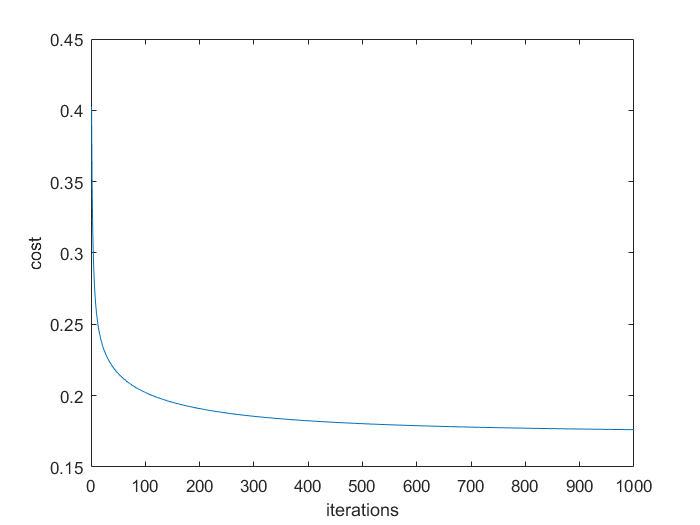
\includegraphics[scale=0.4]{cost.png}
	\caption{针对第一类进行训练时梯度下降的收敛情况}
	\label{fig:label}
\end{figure}\\
\noindent\textbf{实验结果}\\
对于训练集的预测准确度达到了0.94,对于测试集的预测准确度到达了0.91,预测的结果综合来看比较乐观。\\\\

\noindent\textbf{附加题目}\\
我额外做了一些实验来测试一下策略:\\
1. 对多数类使用欠采样,适当减少多数类数量\\
2. 对少数类过采样的时候适当减少采样倍数,这样可以提高少数类的查准率\\
综合上述策略,采用的设置为:数目最多的类别(第一类)随机减少一半样本,少数类在过采样时将样本数量扩展到多数类数量的5分之一。\\
按照上述设置进行实验,得出结果为表4所示,发现测试集准确率,少数类查准率有了上升\\
\begin{table}[!h]
	\centering
	\caption{添加欠采样,同时降低少数类过采样倍数的实验结果}\vspace{3mm}
	\label{new_exp_performance}
	\begin{tabular}{@{}c|cccccc@{}}
		\toprule
		标记     & 1    & 2    & 3    & 4    & 5    & \begin{tabular}[c]{@{}c@{}}准确率\end{tabular} \\ \midrule
		查全率    & 0.97 & 0.75 & 0.75 & 0.67 & 0.42 & \multirow{2}{*}{0.94}                                     \\
		查准率 & 0.96 & 0.93 & 1.00 & 1.00 & 0.45 &  \\ \cmidrule(r){1-7}
	\end{tabular}
\end{table}\\
但是在这种设置下训练集上的准确率发生了明显的下降,同时程序的结果也不如之前的设置稳定。对此作出的推测为:欠采样的随机性太强,减少了很多多数类的样本,有可能丢掉了一些“关键”的样本,所以分类器在训练集的预测效果下降。至于少数类的查准率上升有可能就是因为过采样生成样本数量较少导致的。\\
考虑到新的设置在训练集上效果变差,而且不是非常稳定,随机性较强,\textbf{所以最终提交的代码还是保持了原来的设置,即,仅使用了smote过采样算法,不再使用欠采样。}\\\\
附加实验参考资料:\\
1. Zhi-Hua Zhou (2016) 机器学习\\
2. V. Chawla, Kevin W. Bowyer, Lawrence O. Hall, W. Philip Kegelmeyer (2002) SMOTE: Synthetic Minority Over-sampling Technique Nitesh \\\\
\noindent\textbf{实验心得}\\
\begin{itemize}
\item 对于少数类别的处理非常重要,提高少数类别的准确率也很不容易。
\item 选择不同的优化算法会显著影响结果收敛与否,收敛速度。 
\item 如何处理不同特征之间范围差异过大的问题也会影响算法的性能。
\item matlab程序的编写和c++还是有很大不同,想要灵活熟练运用matlab还需要大量的积累和练习。
\end{itemize}
~\\
\noindent\textbf{参考资料}\\
1. Zhi-Hua Zhou (2016) 机器学习\\
2. V. Chawla, Kevin W. Bowyer, Lawrence O. Hall, W. Philip Kegelmeyer (2002) SMOTE: Synthetic Minority Over-sampling Technique Nitesh \\
\end{document}